% Source-SHA256: 7773a799071b3e1b5d9bddf93d59cba48bcdef018cd698cdd190ea90a44e8d79
% !TeX program = xelatex
\documentclass[a4paper,11pt]{article}
\usepackage{fontspec}
\IfFontExistsTF{TeX Gyre Pagella}{\setmainfont{TeX Gyre Pagella}}{\setmainfont{P052}}
\IfFontExistsTF{TeX Gyre Heros}{\setsansfont{TeX Gyre Heros}}{\setsansfont{Nimbus Sans}}
\IfFontExistsTF{TeX Gyre Cursor}{\setmonofont{TeX Gyre Cursor}[Scale=0.88]}{\setmonofont{Nimbus Mono PS}[Scale=0.88]}
\usepackage{babel}
\babelprovide[import,main]{spanish}
\usepackage{microtype}
\usepackage[a4paper,margin=2.6cm,headheight=23pt,headsep=10pt,footskip=1.1cm]{geometry}
\raggedbottom
\setlength{\emergencystretch}{3em}
\hyphenpenalty=10000
\exhyphenpenalty=10000
\clubpenalty=10000
\widowpenalty=10000
\usepackage{xcolor}
\definecolor{navybg}{HTML}{0B1D2E}
\definecolor{navydeep}{HTML}{123049}
\definecolor{lightblue}{HTML}{8FD3FE}
\definecolor{amber}{HTML}{F5A623}
\definecolor{softgray}{HTML}{5B6570}
\usepackage{titlesec,needspace}
\titleformat{\section}{\sffamily\Large\bfseries\color{navydeep}\raggedright}{\thesection}{10pt}{}
\titleformat{\subsection}{\sffamily\large\bfseries\color{navydeep}\raggedright}{\thesubsection}{8pt}{}
\titlespacing*{\section}{0pt}{20pt}{9pt}
\usepackage{fancyhdr}
\pagestyle{fancy}
\fancyhf{}
\fancyhead[C]{\small\sffamily\color{softgray}Drop Route --- Diseño Técnico del Software}
\fancyfoot[L]{\small\sffamily\color{softgray}Base reconstruida · 13/10/2026}
\fancyfoot[R]{\small\sffamily\color{softgray}\thepage}
\renewcommand{\headrulewidth}{0.4pt}
\usepackage{array,longtable,booktabs,calc}
\renewcommand{\arraystretch}{1.15}
\usepackage{enumitem}
\setlist[itemize]{leftmargin=1.4em,itemsep=3pt,topsep=5pt}
\usepackage{fancyvrb,framed,seqsplit}
\let\originaltexttt\texttt
\renewcommand{\texttt}[1]{\originaltexttt{\seqsplit{#1}}}
\providecommand{\tightlist}{\setlength{\itemsep}{2pt}\setlength{\parskip}{0pt}}
\usepackage{graphicx,tikz,xurl}
\usepackage[colorlinks=true,linkcolor=navydeep,urlcolor=navydeep,bookmarksnumbered=true,pdftitle={DTS - Drop Route},pdfauthor={Jesús Quevedo Rodríguez}]{hyperref}
\usepackage{bookmark}
\setlength{\parindent}{0pt}
\setlength{\parskip}{6pt}
\begin{document}
\begin{titlepage}
\newgeometry{margin=0cm}
\thispagestyle{empty}
\begin{tikzpicture}[remember picture,overlay]
\fill[navybg] (current page.south west) rectangle (current page.north east);
\node[anchor=north,text width=16cm,align=center] at ([yshift=-3.3cm]current page.north) {\sffamily\bfseries\fontsize{16}{19}\selectfont\color{amber}DROP ROUTE};
\node[anchor=north,text width=16cm,align=center] at ([yshift=-5cm]current page.north) {\sffamily\bfseries\fontsize{30}{38}\selectfont\color{white}Documento de Diseño\\Técnico del Software};
\node[anchor=north,text width=14cm,align=center] at ([yshift=-9.2cm]current page.north) {\sffamily\fontsize{14}{20}\selectfont\color{lightblue}Voicings de guitarra y rutas II--V--I\\Base de desarrollo para Claude Code};
\begin{scope}[shift={([xshift=2.4cm,yshift=7.7cm]current page.south west)}]
\foreach \y in {0,0.5,1,1.5,2,2.5} {\draw[white,opacity=0.28,line width=0.7pt] (0,\y)--(16,\y);}
\foreach \x in {0,2.5,5,7.5,10,12.5,15} {\draw[lightblue,opacity=0.25] (\x,0)--(\x,2.5);}
\fill[amber] (3.75,1) circle (0.2);
\fill[lightblue] (8.75,1.5) circle (0.2);
\fill[white] (8.75,2) circle (0.2);
\fill[lightblue] (8.75,2.5) circle (0.2);
\end{scope}
\node[anchor=south west,text width=16cm,align=left] at ([xshift=2.4cm,yshift=2cm]current page.south west) {\sffamily\fontsize{11}{17}\selectfont\color{white}\textcolor{amber}{Autor del proyecto:} Jesús Quevedo Rodríguez\\\textcolor{amber}{Revisión:} base reconstruida · 13/10/2026\\\textcolor{amber}{Repositorio:} a01653/Drop\_Route\\\textcolor{amber}{Estado:} juego pendiente de implementación};
\end{tikzpicture}
\end{titlepage}
\restoregeometry
\tableofcontents
\newpage
\Needspace{4cm}
\hypertarget{objetivo-y-alcance}{%
\section{Objetivo y alcance}\label{objetivo-y-alcance}}

Drop Route servirá para memorizar voicings, inversiones y grados y
practicar rutas II-V-I concretas. Ordenador y móvil. Primera etapa en C,
con la apariencia de nuestras tarjetas.

Se preparan fuentes e instrucciones para que Claude Code implemente cada
etapa mediante órdenes de trabajo. No necesita acceder al historial de
esta conversación ni recibir las plantillas de nuevo.

\Needspace{4cm}
\hypertarget{arquitectura-general}{%
\section{Arquitectura general}\label{arquitectura-general}}

Diseño previsto de aplicación cliente, sin backend.

\begin{longtable}[]{@{}>{\raggedright\arraybackslash}p{\dimexpr0.290000\linewidth-1.000000\tabcolsep\relax}>{\raggedright\arraybackslash}p{\dimexpr0.710000\linewidth-1.000000\tabcolsep\relax}@{}}
\toprule\noalign{}
Capa & Responsabilidad prevista \\
\midrule\noalign{}
\endhead
\bottomrule\noalign{}
\endlastfoot
Datos & Posiciones y rutas procedentes de la plantilla. \\
Núcleo musical & Alturas físicas, grados, inversiones y solución de
ruta. \\
Sesión & Pregunta, selección, evaluación y transición. \\
Presentación & Tarjeta SVG, selectores, fichas y resultados. \\
Persistencia & Configuración y progreso local con versión de esquema. \\
\end{longtable}

La geometría no decide la respuesta y los componentes no duplican el
catálogo. Actualmente están implementados la extracción y el núcleo de
auditoría de esta base, no el motor del juego.

\Needspace{4cm}
\hypertarget{tecnologuxedas-y-dependencias}{%
\section{Tecnologías y
dependencias}\label{tecnologuxedas-y-dependencias}}

Node.js 22 o superior ejecuta tests y auditorías. Python 3.10 o superior
extrae las constantes literales. La base no necesita dependencias npm
externas.

DR-001 propone React, TypeScript y Vite; ESLint, Vitest y Playwright.
Elegir y fijar versiones compatibles al ejecutar esa tarea. No copiar
dependencias innecesarias de Mástil.

Pandoc y LuaLaTeX completo o XeLaTeX generan este documento. El estilo
utiliza la paleta azul oscuro y familias tipográficas de la
documentación de Mástil, con equivalentes si faltan TeX Gyre. Idioma
español y sin partición de palabras al final de línea.

\Needspace{4cm}
\hypertarget{estructura-actual}{%
\section{Estructura actual}\label{estructura-actual}}

\begin{longtable}[]{@{}>{\raggedright\arraybackslash}p{\dimexpr0.290000\linewidth-1.000000\tabcolsep\relax}>{\raggedright\arraybackslash}p{\dimexpr0.710000\linewidth-1.000000\tabcolsep\relax}@{}}
\toprule\noalign{}
Ruta & Contenido \\
\midrule\noalign{}
\endhead
\bottomrule\noalign{}
\endlastfoot
\texttt{CLAUDE.md} / \texttt{AGENTS.md} & Reglas permanentes y flujo de
trabajo. \\
\texttt{data/catalog.json} & Sets, fórmulas, afinación y 124 formas. \\
\texttt{data/routes.json} & Dieciséis rutas II-V-I completas. \\
references/ & Tres fuentes originales y sus hashes. \\
scripts/ & Extracción, auditoría y generación documental. \\
tests/ & Pruebas ejecutables de la base. \\
e2e/ & Nota de alcance; aún no hay specs ejecutables. \\
docs/ & Requisitos, decisiones, tareas, validación y DTS. \\
.github/workflows/ & Validación de la base preparada para GitHub. \\
\end{longtable}

No hay src o build web en esta revisión. La estructura de interfaz se
establece en DR-001.

\Needspace{4cm}
\hypertarget{componentes-previstos}{%
\section{Componentes previstos}\label{componentes-previstos}}

\begin{longtable}[]{@{}>{\raggedright\arraybackslash}p{\dimexpr0.290000\linewidth-1.000000\tabcolsep\relax}>{\raggedright\arraybackslash}p{\dimexpr0.710000\linewidth-1.000000\tabcolsep\relax}@{}}
\toprule\noalign{}
Componente & Responsabilidad \\
\midrule\noalign{}
\endhead
\bottomrule\noalign{}
\endlastfoot
Configuración & Juego, Drop, set, dificultad y modo de ruta. \\
Tarjeta & Cuerdas, trastes, notas y estado neutro/solución. \\
Respuesta & Cuatro botones o dos desplegables. \\
Grados & Cuatro destinos, arrastre, dos toques y teclado. \\
Rutas & Partida fija y una candidata visible. \\
Corrección & Resultado por campos y avance explícito. \\
\end{longtable}

Compartir el renderizador conserva proporciones entre juegos. El icono
final sigue pendiente; el brief está en \texttt{docs/VISUAL.md}.

\Needspace{4cm}
\hypertarget{estado-y-persistencia}{%
\section{Estado y persistencia}\label{estado-y-persistencia}}

Modelo previsto: configuración, pregunta, pregunta verificada y regreso
al menú. Cada pregunta identifica datos y guarda sus opciones y orden.

Seleccionar no evalúa. Verificar exige respuesta completa y produce un
único resultado. Después se bloquea la respuesta. Siguiente genera otra
pregunta y Salir vuelve al menú.

La corrección no sobrescribe lo que contestó el usuario. Si falla el V
de una ruta, el paso V-I debe partir del V correcto.

DR-006 añadirá progreso local con esquema independiente de la versión de
app. Ninguna persistencia está implementada todavía.

\Needspace{4cm}
\hypertarget{modelo-musical}{%
\section{Modelo musical}\label{modelo-musical}}

Afinación estándar EADGBE. MIDI al aire, cuerdas 6 a 1:
40,45,50,55,59,64. Altura real igual a MIDI al aire más traste.

Calidades evaluables en C: maj7 (0,4,7,11), 7 (0,4,7,10), m7 (0,3,7,10)
y m7(b5) (0,3,6,10). Grados reales, incluidas b3, b5 y b7.

Inversión por bajo real: raíz, tercera, quinta o séptima. No deducirla
del primer elemento de un array.

Cdim7 se conserva como referencia: 0,3,6,9 y bb7. La fuente rotula su
séptima como °7. El acorde es simétrico y no se evalúa sin fijar raíz y
contexto.

\Needspace{4cm}
\hypertarget{catuxe1logo-y-construcciuxf3n-de-voicings}{%
\section{Catálogo y construcción de
voicings}\label{catuxe1logo-y-construcciuxf3n-de-voicings}}

No se generan posiciones nuevas. Drop 2 tiene tres sets; Drop 3 y Drop
2+4, dos cada uno. Cuatro calidades y cuatro inversiones dan 112
posiciones evaluables. Hay otras doce disminuidas de referencia.

La auditoría verifica cuerda/traste, fórmula, grados, bajo y orden por
Drop. La extracción analiza datos literales sin ejecutar JavaScript.
-\/-check confirma que los JSON coinciden con la fuente sin
sobrescribir.

Mantener ventana corta de las tarjetas. Algunas formas abarcan cinco
trastes: no recortar para imponer una ventana de tres.

\Needspace{4cm}
\hypertarget{rutas-y-conducciuxf3n-de-voces}{%
\section{Rutas y conducción de
voces}\label{rutas-y-conducciuxf3n-de-voces}}

Normalizadas solo Drop 2 sets 1 y 2, mayor y menor, cuatro inversiones
iniciales: dieciséis rutas.

\begin{longtable}[]{@{}>{\raggedright\arraybackslash}p{\dimexpr0.333333\linewidth-1.333333\tabcolsep\relax}>{\raggedright\arraybackslash}p{\dimexpr0.333333\linewidth-1.333333\tabcolsep\relax}>{\raggedright\arraybackslash}p{\dimexpr0.333333\linewidth-1.333333\tabcolsep\relax}@{}}
\toprule\noalign{}
II & V & I \\
\midrule\noalign{}
\endhead
\bottomrule\noalign{}
\endlastfoot
Fundamental & 2ª & Fundamental \\
1ª & 3ª & 1ª \\
2ª & Fundamental & 2ª \\
3ª & 1ª & 3ª \\
\end{longtable}

Mayor Dm7-G7-Cmaj7. Menor Dm7(b5)-G7-Cm7. Comparar con la ruta exacta
del material. Otra inversión de G7 puede ser musicalmente válida y no
corresponder a este ejercicio.

No aplicar un optimizador que sustituya estas rutas ni afirmar mínimo
universal. C6 aparece como sustitución opcional en ciertos pasos de la
fuente; no se convierte automáticamente en otro acorde evaluable.

\Needspace{4cm}
\hypertarget{preguntas-y-correcciuxf3n}{%
\section{Preguntas y corrección}\label{preguntas-y-correcciuxf3n}}

Diseño acordado: fácil elige nombre con cuatro botones; medio añade
inversión en un segundo desplegable; difícil añade colocar grados sobre
círculos.

Opciones únicas y una correcta. En tests, fixture o semilla
reproducible. El banco difícil es fijo con alteraciones y distractores;
ofrecer solo los grados correctos daría una pista.

Corrección por acorde, inversión y cada destino. Acierto completo exige
todos los campos del nivel. Registrar una sola respuesta por primer
intento y bloquear cambios al verificar.

\Needspace{4cm}
\hypertarget{muxf3vil-y-accesibilidad}{%
\section{Móvil y accesibilidad}\label{muxf3vil-y-accesibilidad}}

El fondo es el tramo corto de mástil de las tarjetas, no un mástil
completo de doce trastes. En rutas, partida arriba, candidata debajo y
selector 1/2/3/4; no cuatro candidatas pequeñas simultáneas.

Pregunta con círculos grises y fondo común. No revelar solución mediante
nombre, título, tooltip o nombre accesible de las opciones. Al corregir,
recuperar colores musicales y usar texto/símbolos además de rojo/verde.

Arrastre con tolerancia, alternativa de tocar ficha y destino y
operación por teclado. Áreas táctiles mayores que los círculos visibles.
Se prevén E2E a 360,390 y 430 px; aún no ejecutables.

\Needspace{4cm}
\hypertarget{offline-e-instalaciuxf3n}{%
\section{Offline e instalación}\label{offline-e-instalaciuxf3n}}

DR-006 prevé PWA instalable, caché de recursos propios y recarga sin
conexión tras una primera carga completa.

Progreso por dispositivo, sin sincronización, cuentas, backend o
notificaciones. Probar almacenamiento bloqueado, datos dañados y
migración. No hay manifest PWA, service worker o instalación comprobada
todavía.

\Needspace{4cm}
\hypertarget{documentaciuxf3n-y-claude}{%
\section{Documentación y Claude}\label{documentaciuxf3n-y-claude}}

\texttt{CLAUDE.md} importa \texttt{AGENTS.md} y dirige al contrato y a
la orden solicitada. Las reglas permanentes están versionadas. Las
tareas concretas se describen en DR-001 a DR-007 y se ejecutan por
separado.

Se adapta el flujo de Mástil Escalas: rama por objetivo, pruebas
dirigidas durante ajustes, revisión funcional y batería final aplicable.
Un cambio material de diseño actualiza el DTS principal y sus derivados
en la misma rama.

La preparación se conserva como paquete duradero. El 13/10/2026 el
usuario autorizó la publicación de la base completa en el repositorio
público, incluidos los originales.

\Needspace{4cm}
\hypertarget{flujo-de-datos}{%
\section{Flujo de datos}\label{flujo-de-datos}}

Previsto: configuración selecciona registros; generador crea pregunta
estable; tarjeta dibuja geometría; el usuario compone respuesta;
evaluador calcula resultado según contrato.

En rutas, pregunta identifica ruta y paso. Cambiar candidata no cambia
la partida. El estado de selección no altera los datos musicales.

La futura sesión y el núcleo musical deben poder probarse sin DOM; los
componentes consumen el catálogo sin duplicar posiciones.

\Needspace{4cm}
\hypertarget{pruebas-y-resultados-reales}{%
\section{Pruebas y resultados
reales}\label{pruebas-y-resultados-reales}}

La reconstrucción ha ejecutado 24 tests con node:test: todos pasan, sin
omitidos. Verifican catálogo completo, rutas, hashes de fuentes y
rechazo de errores deliberados.

La auditoría pasa con 124 posiciones (112 evaluables y doce de
referencia) y 16 rutas. Hay oráculos independientes para D2S1 mayor
primera inversión y D2S2 menor fundamental.

Se prueba también una forma G7 válida en otra inversión que no cumple la
ruta. Los tests no se limitan a comparar las tablas consigo mismas.

Vitest, lint, build web y Playwright se incorporarán en DR-001. Estos
resultados no se presentan como cobertura del juego, que todavía no
existe.

\Needspace{4cm}
\hypertarget{construcciuxf3n-y-publicaciuxf3n}{%
\section{Construcción y
publicación}\label{construcciuxf3n-y-publicaciuxf3n}}

npm run docs:build regenera LaTeX/PDF desde el Markdown. Guarda hashes
del Markdown, derivados, plantilla y generador para detectar
desactualizaciones.

La CI preparada ejecuta npm ci y npm run validate. Esta revisión del DTS
es previa a la publicación inicial; su ejecución remota se comprobará
después del push. El código en Git tampoco equivale a tener el juego
desplegado.

El primer push fue bloqueado por revisión automática debido al
repositorio público y los materiales originales. El 13/10/2026 se obtuvo
autorización explícita del usuario para publicar la base completa. Las
futuras publicaciones siguen requiriendo una orden que las cubra.

\Needspace{4cm}
\hypertarget{limitaciones-actuales}{%
\section{Limitaciones actuales}\label{limitaciones-actuales}}

\begin{itemize}
\tightlist
\item
  No existe aún interfaz, icono final, progreso, PWA o revisión
  funcional móvil.
\item
  Solo se normalizaron las rutas Drop 2 sets 1 y 2 del HTML.
\item
  Los PDF tienen 21 páginas de imágenes cada uno; no se han transcrito
  íntegramente.
\item
  Cdim7 y C6 no son calidades evaluables de la primera etapa.
\item
  Transposición y audio quedan para otra etapa.
\item
  La reconstrucción conserva contratos y datos, no recupera el commit
  local perdido byte a byte.
\item
  Hosting y licencia del código nuevo pendientes; las referencias
  conservan su autoría.
\end{itemize}

\Needspace{4cm}
\hypertarget{evoluciuxf3n}{%
\section{Evolución}\label{evoluciuxf3n}}

DR-001 configura herramientas; DR-002 crea tarjetas e icono; DR-003 y
DR-004, reconocimiento; DR-005, rutas; DR-006, progreso/PWA; DR-007,
cierre documental y pruebas.

Convertir lo planificado en descripción de implementación solo después
de inspeccionar y probar el código. No extender una tarea a mejoras no
pedidas.

\Needspace{4cm}
\hypertarget{apuxe9ndice-evidencia-y-luxedmites}{%
\section{Apéndice: evidencia y
límites}\label{apuxe9ndice-evidencia-y-luxedmites}}

Verificados: mismas tres referencias, SHA-256, extracción, notas
físicas, fórmulas, grados, inversiones, rutas y 24 tests ejecutados
nuevamente. Documentación reconstruida desde las decisiones visibles de
la conversación.

No se ha ejecutado Claude Code en el equipo del usuario ni implementado
el juego. Esta revisión documenta el candidato anterior a la publicación
inicial autorizada. La compilación del DTS, revisión visual y validación
documental se registran en
\texttt{docs/validation/2026-10-13-foundation.md}.
\end{document}
